\subsection{RQ3: To what extent can specialized SLMs improve the detection of errors in generated code?}
\label{sec:rq3}

\begin{figure}[htbp]
\centering
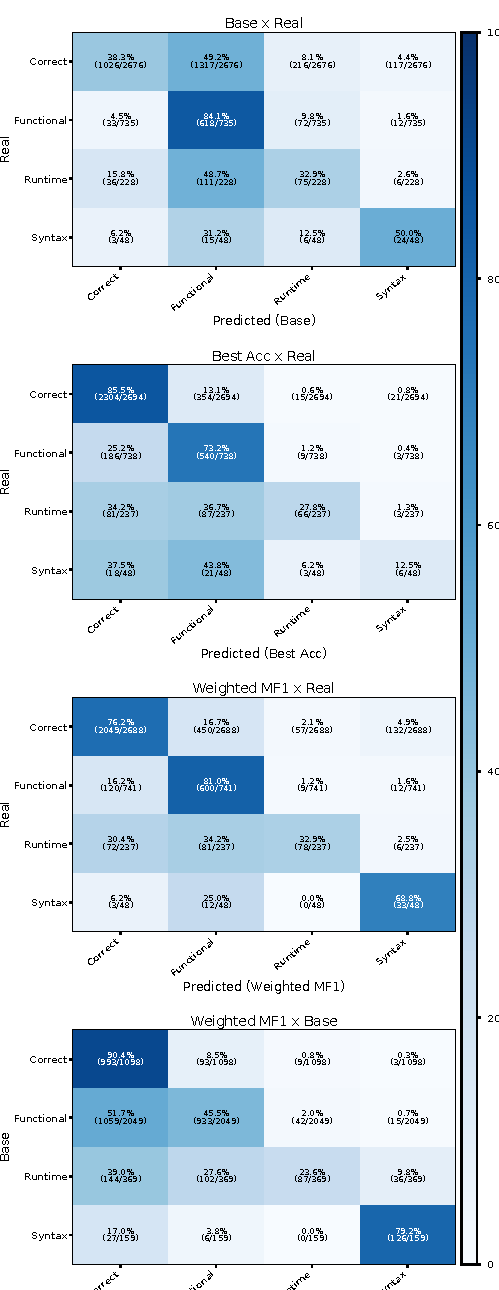
\includegraphics[width=\columnwidth]{figures/confusion_matrices.pdf}
\caption{Row-normalized confusion matrices under a primary-label reduction (priority syntax, runtime, functional, correct). Each cell reports the proportion and the counts as predicted / reference total. The first three matrices use the ground truth as reference, and the last compares the Weighted MF1 predictions against the base predictions. The number of evaluated samples differs slightly across matrices (Base 3{,}687; Best Acc 3{,}717; Weighted MF1 3{,}714; Weighted MF1 vs Base 3{,}675) because unparsable model outputs were excluded from the primary-label reduction.}
\label{fig:confusion}
\end{figure}

The dataset used for training is strongly imbalanced. Correct samples represent 72.4\% of the records, followed by Functional Error with 21.3\%, Runtime Error with 6.6\%, and Syntax Error with only 1.5\%. Because Accuracy favors predictions of the dominant class, a model trained on this distribution can learn to play safe and predict Correct most of the time. This motivated the evaluation of different training strategies. The split is performed at the task level, so all samples of a given programming task belong to a single split, and balancing is applied only to the training split, while validation and test remain intact.

The first search optimized validation Accuracy using the standard causal loss and the original class distribution. The search explored the base model, LoRA rank, alpha, dropout, learning rate, epochs, and bias configuration. The best configuration used Gemma 4 E4B with $r=16$, $\alpha=16$, dropout 0.1, learning rate $1\times10^{-4}$, 3 epochs, and bias \texttt{none}, reaching a validation Accuracy of 66.6\%. Figure~\ref{fig:confusion} shows that the Accuracy-oriented model shifts its decision boundary toward the dominant Correct class. In the base model, only 38.3\% of the Correct samples remain Correct, while 49.2\% are confused with Functional. Best Acc reduces Correct to Functional from 49.2\% to 13.1\% and also reduces Correct to Runtime (8.1\% to 0.6\%) and Correct to Syntax (4.4\% to 0.8\%), which explains where the Accuracy gain comes from. The cost is visible in the reverse direction: Functional to Correct rises from 4.5\% to 25.2\%, Runtime to Correct from 15.8\% to 34.2\%, and Syntax to Correct from 6.2\% to 37.5\%. The model did not simply learn Correct better; it began to favor Correct as an output.

Because per-class performance remained unbalanced, a second search optimized Macro-F1 instead. This search kept the same data distribution without explicit balancing and used the \texttt{label\_weighted} strategy with a class weight of 3.0. The best configuration used Gemma 4 E4B with $r=8$, $\alpha=8$, dropout 0.1, learning rate $1\times10^{-4}$, 3 epochs, and bias \texttt{none}, reaching a validation Macro-F1 of 52.4\% and a validation Macro Recall of 54.9\%.

The comparison between the two optimization objectives, presented in Table~\ref{tab:rq2_detection} and in Figure~\ref{fig:confusion}, clarifies how strongly the training objective changes the detector profile. Best Acc maximizes global performance, with 77.8\% Accuracy, 50.9\% Macro-F1, and 85.5\% Correct Recall. Weighted MF1 reduces Correct Recall to 76.2\% but increases Functional Recall from 73.2\% to 81.0\%, Runtime Recall from 27.8\% to 32.9\%, and Syntax Recall from 12.5\% to 68.8\%. The confusion matrices show that Weighted MF1 also reduces the tendency of Best Acc to absorb minority classes into Correct: Functional to Correct falls from 25.2\% to 16.2\%, and Syntax to Correct falls from 37.5\% to 6.2\%. In contrast to Best Acc, the Macro-F1-oriented model partially reverses the tendency to collapse minority classes into Correct. The optimization objective therefore changes not only the aggregate score but the classes the detector learns to recognize, and this is one of the main findings of this RQ.

Runtime remains the least stable class across training strategies. In the base model, Runtime is predicted as Functional in 48.7\% of cases and as Runtime in 32.9\%. Best Acc shifts Runtime toward Correct (34.2\%) and keeps only 27.8\% as Runtime, while Weighted MF1 keeps 32.9\% as Runtime and sends 30.4\% to Correct and 34.2\% to Functional. Fine-tuning changes where Runtime samples are misclassified, but does not produce an improvement comparable to that observed for Correct or Syntax. Syntax, in turn, is highly sensitive to the training strategy: it ranges from 11.8\% recall under Accuracy-oriented training to 64.7\% under Macro-F1-oriented training.

A third strategy changed the training distribution itself, reducing the number of Correct examples, removing Syntax, and testing proportions such as 1:1:1 and 1:3:3, with the goal of increasing the relative representation of the minority classes. The Balanced Acc model reached 67.8\% Accuracy, 38.1\% Macro-F1, 74.4\% Correct Recall, 65.8\% Functional Recall, 15.2\% Runtime Recall, and 0\% Syntax Recall. The Balanced MF1 model reached 63.7\% Accuracy, 36.0\% Macro-F1, 68.6\% Correct Recall, 65.8\% Functional Recall, 13.9\% Runtime Recall, and 0\% Syntax Recall.

Explicit balancing did not outperform the previous strategies. Both Accuracy and Macro-F1 decreased, Runtime detection also degraded, and Syntax reached 0\% because the class was removed from training. This suggests that simply rebalancing examples does not guarantee better learning, and that removing Correct examples may discard important information about the dominant class. In this setting, changing the objective and the loss was more effective than changing the dataset distribution. Objective-oriented training was more effective than explicit dataset balancing.

Syntax deserves separate discussion. The class is extremely rare, and many cases classified as Syntax result from an incompatible output format or structure rather than syntactically invalid Python. This makes the class small, heterogeneous, and difficult to learn, and highly sensitive to the training objective. The results illustrate this sensitivity: Best Acc reached 11.8\% Syntax Recall, Weighted MF1 reached 64.7\%, and the balanced models reached 0\%. These cases are not reclassified; the observed behavior only reflects how the training strategy interacts with a rare and heterogeneous class.

The overall effect of fine-tuning can be summarized by comparing the base and specialized models. The Gemma 4 E4B base model obtained 45.9\% Accuracy and 37.0\% Macro-F1. The Best Acc model reached 77.8\% Accuracy and 50.9\% Macro-F1, while Weighted MF1 reached 73.5\% Accuracy and 54.2\% Macro-F1. Fine-tuning therefore produces a substantial gain, and the specialization strongly changes the ability to recognize Correct, with Weighted MF1 producing the most balanced detector and Best Acc producing the strongest Accuracy. The deltas relative to the base model confirm this effect: Best Acc gains 31.9 percentage points of Accuracy, 13.9 of Macro-F1, and 47.3 of Correct Recall, while losing 17.3 of Functional Recall and 35.3 of Syntax Recall. Weighted MF1 gains 27.6 of Accuracy, 17.2 of Macro-F1, 37.9 of Correct Recall, and 17.6 of Syntax Recall. The balanced models gain around 21.9 and 17.8 of Accuracy but lose more than 20 points of Functional Recall and 47 of Syntax Recall.

The last matrix in Figure~\ref{fig:confusion} compares the Weighted MF1 predictions directly against the base predictions and should be interpreted as a prediction transition, not as correctness. It shows that among the samples the base model labeled as Correct, 90.4\% remain Correct; among those labeled as Functional, 51.7\% are reclassified as Correct by Weighted MF1; among those labeled as Runtime, only 23.6\% remain Runtime; and among those labeled as Syntax, 79.2\% remain Syntax. The largest behavioral shift therefore occurs among samples originally labeled as Functional by the base model, which are frequently reclassified as Correct. This does not imply an error by itself; it only shows how the decision behavior changed. Fine-tuning does not simply improve the detector: it changes its decision behavior, and different optimization objectives produce distinct error profiles.

\textbf{Answer to RQ3.} Specialized training substantially improves SLM-based error detection, but the resulting detector is highly sensitive to the optimization objective and to the class-imbalance strategy. Accuracy-oriented fine-tuning favors the dominant Correct class, whereas Macro-F1-oriented training yields more balanced performance across error categories. Explicit dataset balancing did not outperform objective-based weighting in the evaluated setting.
